\section{Message passing}
\label{sec:message-passing}
\subsection{TrueSkill latent variable models}
\textbf{Latent variables} are variables that can only be inferred indirectly through a mathematical model from other observable variables that can be directly observed or measured.\\
\newline
\textbf{TrueSkill} model is a player ranking system for competitive games. Our goal is to infer the skills of players in a competitive game, based on the results of the games. Hence, each player's skill is a \textbf{latent variable}, and we assume they are fixed. Moreover, we also assume each player's skill is independent such as independent Gaussian prior.\\
\newline
For each game, the probability that player $i$ beats player $j$ is
$$p(i\:\text{beats}\:j)=\sigma(z_i-z_j),\:\text{where}$$
$$\sigma{(y)}=\frac{1}{1+\text{exp}(-y)}$$
Hence the entire joint likelihood of players and games is:
\begin{gather*}
    p\left(z_1, z_2, \ldots z_N, \text { game } 1, \text { game } 2, . . \text { game } T\right) \\
    =\underbrace{\left[\prod_{i=1}^N p\left(z_i\right)\right]}_{\text{prior}} \underbrace{\left[\prod_{\text {games }} p\left(\mathrm{i} \text { beats } \mathrm{j} \mid z_i, z_j\right)\right]}_{\text{likelihood}}
\end{gather*}
However, it is hard to compute the posterior
\begin{align*}
    & p\left(z_1, z_2 \mid \text { game } 1 \text {, game } 2, \ldots \text { game } T\right) \\
    = & \int \cdots \int p\left(z_1, z_2, z_3 \ldots z_N \mid x\right) d z_3 \ldots d z_N
\end{align*}
\textbf{Message passing} can help us to compute the posterior.

\subsection{Message Passing}
From the last section, we can see that determining an optimal elimination order is hard, and the resulting marginalization can be still costly. Therefore, we introduce the tress as any elimination ordering from leaves to the root is optimal.
\subsubsection*{Inference in trees}
A graph is $G=(\mathcal{V},\:\mathcal{E})$, where $\mathcal{V}$ is vertices and $\mathcal{E}$ is edges. A leaf in a tree is the nodes where it has only one neighbor. We can regard a tress as MRFs, with joint distribution:
$$p\left(x_1, x_2, \ldots, x_n\right)=\underbrace{\frac{1}{Z}}_{\text{normalization}}\overbrace{\prod_{i \in \mathcal{V}} \psi\left(x_i\right)}^{\text{nodes}}\underbrace{\prod_{(i, j) \in \mathcal{E}} \psi_{i j}\left(x_i, x_j\right)}_{\text{edges}}$$
\begin{example}
    \begin{figure}[H]
        \centering
        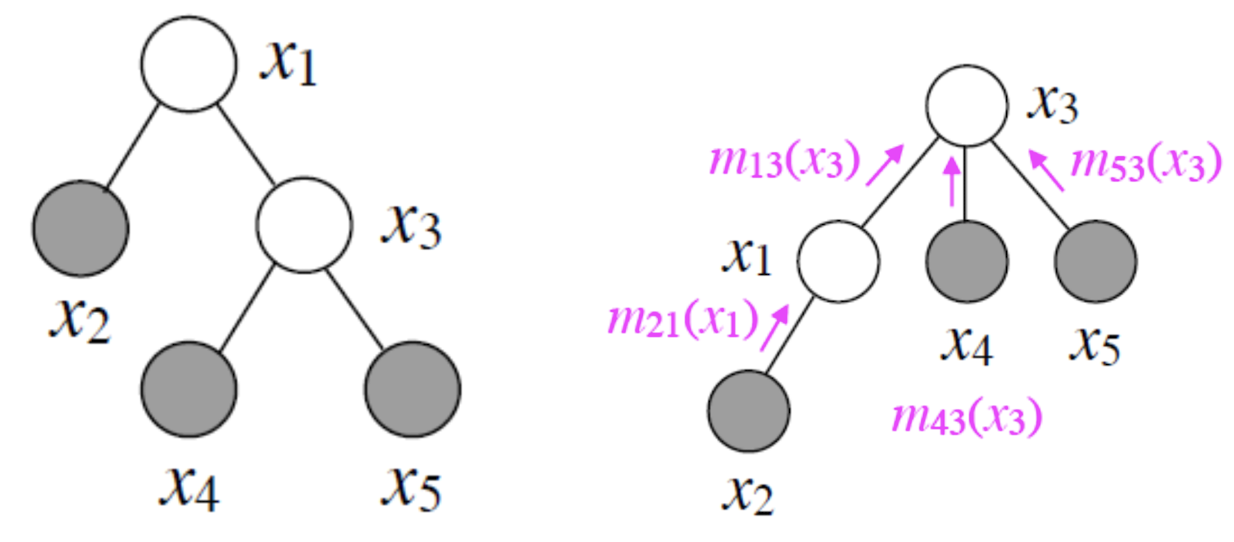
\includegraphics[width = .6\linewidth]{figures/section4/figure_4_1.png}
        \caption{An example of tree and message passing}
        \label{fig:tree}
    \end{figure}
    \hyperref[fig:tree]{Above} shows a tree where $x_E=\{\bar{x_2},\bar{x_4},\bar{x_5}\},\:x_R=x_1$. We want to compute $p(x_3\mid x_E)$:
    \begin{align*}
        p(x_3|x_E)&=\frac{p\left(x_3, x_E\right)}{\sum_{x_3^{\prime}} p\left(x_3^{\prime}, x_E\right)}\\
        &=\frac{1}{Z^E}\:p(x_3,x_E)\\
    \end{align*}
    Express $p(x_3,x_E)$, we have
    \begin{align*}
        &=\sum_{x_1} \psi_1\left(x_1\right) \psi_2\left(\bar{x}_2\right) \psi_3\left(x_3\right) \psi_4\left(\bar{x}_4\right) \psi_5\left(\bar{x}_5\right) \psi_{12}\left(x_1, \bar{x}_2\right) \psi_{13}\left(x_1, x_3\right) \psi_{34}\left(x_3, \bar{x}_4\right) \psi_{35}\left(x_3, \bar{x}_5\right)\\
        &=\frac{1}{Z^E} \underbrace{\psi_4\left(\bar{x}_4\right) \psi_{34}\left(x_3, \bar{x}_4\right)}_{m_{43}\left(x_3\right)} \underbrace{\psi_5\left(\bar{x}_5\right) \psi_{35}\left(x_3, \bar{x}_5\right)}_{m_{53}\left(x_3\right)} \psi_3\left(x_3\right) \sum_{x_1} \psi_1\left(x_1\right) \psi_{13}\left(x_1, x_3\right) \underbrace{\psi_2\left(\bar{x}_2\right) \psi_{12}\left(x_1, \bar{x}_2\right)}_{m_{21}\left(x_1\right)} \\
        &=\frac{1}{Z^E} m_{43}\left(x_3\right) m_{53}\left(x_3\right) \psi_3\left(x_3\right) \underbrace{\sum_{x_1} \psi_1\left(x_1\right) \psi_{13}\left(x_1, x_3\right) m_{21}\left(x_1\right)}_{m_{13}\left(x_3\right)} \\
        &=\frac{1}{Z^E} \psi_3\left(x_3\right) m_{43}\left(x_3\right) m_{53}\left(x_3\right) m_{13}\left(x_3\right)\\
        &=\frac{\psi_3\left(x_3\right) m_{43}\left(x_3\right) m_{53}\left(x_3\right) m_{13}\left(x_3\right)}{\sum_{x_3^{\prime}} \psi_3\left(x_3^{\prime}\right) m_{43}\left(x_3^{\prime}\right) m_{53}\left(x_3^{\prime}\right) m_{13}\left(x_3^{\prime}\right)}
    \end{align*}
\end{example}
\subsubsection*{Sum-product algorithm}
The above example shows how we can pass the message and eventually compute the conditional distribution. For each passed message such as $m_{43}(x_3)$, it uses the sum-product algorithm we introduced in the chapter of \hyperref[sec:sum-product]{exact inference}. To summarize, we have:
\begin{itemize}
    \item If $x_j$ \textbf{unobserved}, the message sent from variable $j$ to $i \in N(j)$ is
    $$
    m_{j \rightarrow i}\left(x_i\right)=\sum_{x_j} \psi_j\left(x_j\right) \psi_{i j}\left(x_i, x_j\right) \prod_{k \in N(j) \backslash i} m_{k \rightarrow j}\left(x_j\right)
    $$
    \item If $x_j$ is \textbf{observed}, the message is
    $$
    m_{j \rightarrow i}\left(x_i\right)=\psi_j\left(\bar{x}_j\right) \psi_{i j}\left(x_i, \bar{x}_j\right) \prod_{k \in N(j) \backslash i} m_{k \rightarrow j}\left(\bar{x}_j\right)
    $$
    \item Once the message passing stage is complete, we can compute our beliefs as
    $$
    b\left(x_i\right)=p\left(x_i \mid x_E\right) \propto \psi_i\left(x_i\right) \prod_{j \in N(i)} m_{j \rightarrow i}\left(x_i\right) .
    $$
\end{itemize}
\subsection{Belief Propagation on Trees}
The above algorithm shows how the message is passed from the leaves to the root. In a formal setting, we have four steps:
\begin{enumerate}
    \item Choose the root $r$ arbitrarily.
    \item Pass the message from leaves to $r$.
    \item \textbf{Pass the message from the root to the leafs}. Note that here we only pass the message from the root to the \textbf{unobserved} nodes.
    \item Compute the beliefs/marginals for all unobserved nodes. 
\end{enumerate}
\begin{example}
    We can still infer the previous example (image), and shows the complete belief propagation process. From \hyperref[fig:tree]{Figure 4.1}, our goal is to compute the beliefs
    $$p(x_3|\bar{x_2},\bar{x_4},\bar{x_5})$$ and $$p(x_1|\bar{x_2},\bar{x_4},\bar{x_5})$$
    \textbf{Step 1}: Choose $x_3$ to be our root.\\
    \textbf{Step 2}: Pass the message from leaves to $x_3$.
    \begin{align*}
        & m_{5 \rightarrow 3}\left(x_3\right)=\psi_5\left(\bar{x}_5\right) \psi_{35}\left(x_3, \bar{x}_5\right) \\
        & m_{2 \rightarrow 1}\left(x_1\right)=\psi_2\left(\bar{x}_2\right) \psi_{12}\left(x_1, \bar{x}_2\right) \\
        & m_{4 \rightarrow 3}\left(x_3\right)=\psi_4\left(\bar{x}_4\right) \psi_{34}\left(x_3, \bar{x}_4\right) \\
        & m_{1 \rightarrow 3}\left(x_3\right)=\sum_{x_1} \psi_1\left(x_1\right) \psi_{13}\left(x_1, x_3\right) m_{2 \rightarrow 1}\left(x_1\right)
        \end{align*}
    \textbf{Step 3}: Pass the message from the root to other unobserved nodes:
    $$m_{3 \rightarrow 1}\left(x_1\right)=\sum_{x_3} \psi_3\left(x_3\right) \psi_{13}\left(x_1, x_3\right) m_{4 \rightarrow 3}\left(x_3\right) m_{5 \rightarrow 3}\left(x_3\right)$$
    \textbf{Step 4}: Calculate the beliefs for $x_1$ and $x_3$.
    \begin{align*}
        & b\left(x_1\right) \propto \psi_1\left(x_1\right) m_{2 \rightarrow 1}\left(x_1\right) m_{3 \rightarrow 1}\left(x_1\right) \\
        & b\left(x_3\right) \propto \psi_3\left(x_3\right) m_{1 \rightarrow 3}\left(x_3\right) m_{4 \rightarrow 3}\left(x_3\right) m_{5 \rightarrow 3}\left(x_3\right)
    \end{align*}
\end{example}
\subsubsection*{Loopy Belief Propagation}
The inference we just introduced has limits that the graph (MRF) must be a tree. However, in most cases such as TrueSkill models, we do not have such prerequisites. What we do instead is to keep passing the message until convergence. This is called the Loopy Belief Propagation. It works as follows:
\begin{itemize}
    \item Initialize all messages uniformly:
    $$
    m_{i \rightarrow j}\left(x_j\right)=(1 / k, \ldots, 1 / k)
    $$
    where $k$ is the number of states $x_j$ can take.
    \item Keep running BP updates until \textbf{the messages} "converges":
    $$
    m_{j \rightarrow i}\left(x_i\right)=\sum_{x_j} \psi_j\left(x_j\right) \psi_{i j}\left(x_i, x_j\right) \prod_{k \in N(j) \backslash i} m_{k \rightarrow j}\left(x_j\right)
    $$
    and (sometimes) normalized for stability.
    \item It will generally not converge, but often works fine.
    \item Compute beliefs $b\left(x_i\right) \propto \psi_i\left(x_i\right) \prod_{j \in N(i)} m_{j \rightarrow i}\left(x_i\right)$.
\end{itemize}
\subsubsection*{Max-product belief propagation}
The main difference between the sum-product and max-product belief propagation is that we are now \textbf{maximizing} over $x_j$ instead of summarizing them.\\
$$
m_{j \rightarrow i}\left(x_i\right)=\max _{x_j} \psi_j\left(x_j\right) \psi_{i j}\left(x_i, x_j\right) \prod_{k \in N(j) \backslash i} m_{k \rightarrow j}\left(x_j\right)
$$
Now the beliefs are called max-marginals:
$$
\hat{b}\left(x_i\right)=\max _{x_i} p\left(x_i, x_{\backslash_i}\right) \propto \psi_i\left(x_i\right) \prod_{j \in N(i)} m_{j \rightarrow i}\left(x_i\right) .
$$
MAP inference: take $\hat{x}_i:=\arg \max _{x_i} \hat{b}\left(x_i\right)$ for all $i \notin E$.\\
\hyperref[example-3]{Here} is a numerical example of message passing.